\documentclass{standalone}
\usepackage{tikz}
\usetikzlibrary{patterns, positioning}

\begin{document}
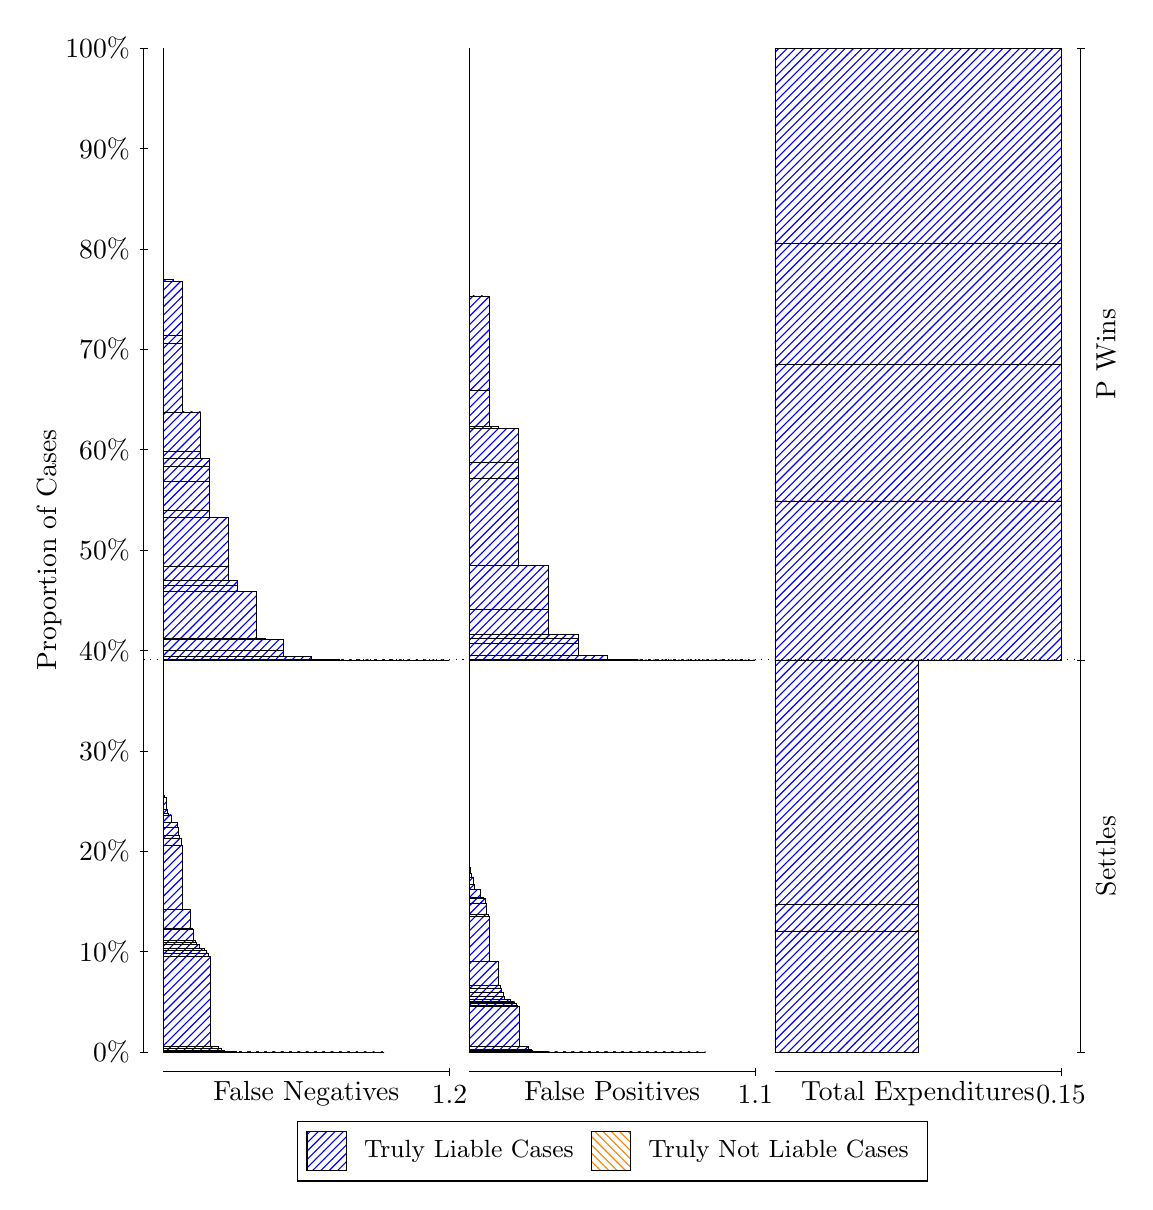
\begin{tikzpicture}
\draw[black, very thin] (1.5,1.75) -- (1.5,14.5);
\node[rotate=90, anchor=center] at (0.3, 8.125) {Proportion of Cases};
\draw[black, very thin] (1.45,1.75) -- (1.55,1.75);
\node[anchor=east] at (1.45, 1.75) {0\%};
\draw[black, very thin] (1.45,3.025) -- (1.55,3.025);
\node[anchor=east] at (1.45, 3.025) {10\%};
\draw[black, very thin] (1.45,4.3) -- (1.55,4.3);
\node[anchor=east] at (1.45, 4.3) {20\%};
\draw[black, very thin] (1.45,5.575) -- (1.55,5.575);
\node[anchor=east] at (1.45, 5.575) {30\%};
\draw[black, very thin] (1.45,6.85) -- (1.55,6.85);
\node[anchor=east] at (1.45, 6.85) {40\%};
\draw[black, very thin] (1.45,8.125) -- (1.55,8.125);
\node[anchor=east] at (1.45, 8.125) {50\%};
\draw[black, very thin] (1.45,9.4) -- (1.55,9.4);
\node[anchor=east] at (1.45, 9.4) {60\%};
\draw[black, very thin] (1.45,10.675) -- (1.55,10.675);
\node[anchor=east] at (1.45, 10.675) {70\%};
\draw[black, very thin] (1.45,11.95) -- (1.55,11.95);
\node[anchor=east] at (1.45, 11.95) {80\%};
\draw[black, very thin] (1.45,13.225) -- (1.55,13.225);
\node[anchor=east] at (1.45, 13.225) {90\%};
\draw[black, very thin] (1.45,14.5) -- (1.55,14.5);
\node[anchor=east] at (1.45, 14.5) {100\%};

\draw[black, very thin] (13.4,1.75) -- (13.4,14.5);
\draw[black, very thin] (13.35,1.75) -- (13.45,1.75);
\node[anchor=west] at (13.35, 1.75) {};
\draw[black, very thin] (13.35,6.7292) -- (13.45,6.7292);
\node[anchor=west] at (13.35, 6.7292) {};
\draw[black, very thin] (13.35,14.5) -- (13.45,14.5);
\node[anchor=west] at (13.35, 14.5) {};

\draw[black, very thin, pattern color=blue, pattern=north east lines] (1.75,1.75) rectangle (4.554,1.75);
\draw[black, very thin, pattern color=blue, pattern=north east lines] (1.75,1.75) rectangle (4.396,1.75);
\draw[black, very thin, pattern color=blue, pattern=north east lines] (1.75,1.75) rectangle (4.238,1.75);
\draw[black, very thin, pattern color=blue, pattern=north east lines] (1.75,1.75) rectangle (4.2029,1.75);
\draw[black, very thin, pattern color=blue, pattern=north east lines] (1.75,1.75) rectangle (4.0801,1.75);
\draw[black, very thin, pattern color=blue, pattern=north east lines] (1.75,1.75) rectangle (4.045,1.75);
\draw[black, very thin, pattern color=blue, pattern=north east lines] (1.75,1.75) rectangle (3.9221,1.75);
\draw[black, very thin, pattern color=blue, pattern=north east lines] (1.75,1.75) rectangle (3.887,1.75);
\draw[black, very thin, pattern color=blue, pattern=north east lines] (1.75,1.75) rectangle (3.8519,1.75);
\draw[black, very thin, pattern color=blue, pattern=north east lines] (1.75,1.75) rectangle (3.7641,1.75);
\draw[black, very thin, pattern color=blue, pattern=north east lines] (1.75,1.75) rectangle (3.729,1.75);
\draw[black, very thin, pattern color=blue, pattern=north east lines] (1.75,1.75) rectangle (3.6939,1.75);
\draw[black, very thin, pattern color=blue, pattern=north east lines] (1.75,1.75) rectangle (3.6062,1.75);
\draw[black, very thin, pattern color=blue, pattern=north east lines] (1.75,1.75) rectangle (3.5711,1.75);
\draw[black, very thin, pattern color=blue, pattern=north east lines] (1.75,1.75) rectangle (3.536,1.75);
\draw[black, very thin, pattern color=blue, pattern=north east lines] (1.75,1.75) rectangle (3.5008,1.75);
\draw[black, very thin, pattern color=blue, pattern=north east lines] (1.75,1.75) rectangle (3.4482,1.75);
\draw[black, very thin, pattern color=blue, pattern=north east lines] (1.75,1.75) rectangle (3.4131,1.75);
\draw[black, very thin, pattern color=blue, pattern=north east lines] (1.75,1.75) rectangle (3.378,1.75);
\draw[black, very thin, pattern color=blue, pattern=north east lines] (1.75,1.75) rectangle (3.3429,1.75);
\draw[black, very thin, pattern color=blue, pattern=north east lines] (1.75,1.75) rectangle (3.2902,1.75);
\draw[black, very thin, pattern color=blue, pattern=north east lines] (1.75,1.75) rectangle (3.2551,1.75);
\draw[black, very thin, pattern color=blue, pattern=north east lines] (1.75,1.75) rectangle (3.22,1.75);
\draw[black, very thin, pattern color=blue, pattern=north east lines] (1.75,1.75) rectangle (3.1849,1.75);
\draw[black, very thin, pattern color=blue, pattern=north east lines] (1.75,1.75) rectangle (3.1498,1.75);
\draw[black, very thin, pattern color=blue, pattern=north east lines] (1.75,1.75) rectangle (3.1322,1.75);
\draw[black, very thin, pattern color=blue, pattern=north east lines] (1.75,1.75) rectangle (3.0971,1.75);
\draw[black, very thin, pattern color=blue, pattern=north east lines] (1.75,1.75) rectangle (3.062,1.75);
\draw[black, very thin, pattern color=blue, pattern=north east lines] (1.75,1.75) rectangle (3.0269,1.75);
\draw[black, very thin, pattern color=blue, pattern=north east lines] (1.75,1.75) rectangle (2.9918,1.75);
\draw[black, very thin, pattern color=blue, pattern=north east lines] (1.75,1.75) rectangle (2.9743,1.7501);
\draw[black, very thin, pattern color=blue, pattern=north east lines] (1.75,1.7501) rectangle (2.9392,1.7501);
\draw[black, very thin, pattern color=blue, pattern=north east lines] (1.75,1.7501) rectangle (2.9041,1.7502);
\draw[black, very thin, pattern color=blue, pattern=north east lines] (1.75,1.7502) rectangle (2.869,1.7503);
\draw[black, very thin, pattern color=blue, pattern=north east lines] (1.75,1.7503) rectangle (2.8339,1.7509);
\draw[black, very thin, pattern color=blue, pattern=north east lines] (1.75,1.7509) rectangle (2.8163,1.7509);
\draw[black, very thin, pattern color=blue, pattern=north east lines] (1.75,1.7509) rectangle (2.7988,1.7514);
\draw[black, very thin, pattern color=blue, pattern=north east lines] (1.75,1.7514) rectangle (2.7812,1.7514);
\draw[black, very thin, pattern color=blue, pattern=north east lines] (1.75,1.7514) rectangle (2.7461,1.7514);
\draw[black, very thin, pattern color=blue, pattern=north east lines] (1.75,1.7514) rectangle (2.711,1.7514);
\draw[black, very thin, pattern color=blue, pattern=north east lines] (1.75,1.7514) rectangle (2.6759,1.7534);
\draw[black, very thin, pattern color=blue, pattern=north east lines] (1.75,1.7534) rectangle (2.6583,1.754);
\draw[black, very thin, pattern color=blue, pattern=north east lines] (1.75,1.754) rectangle (2.6408,1.7559);
\draw[black, very thin, pattern color=blue, pattern=north east lines] (1.75,1.7559) rectangle (2.6232,1.7574);
\draw[black, very thin, pattern color=blue, pattern=north east lines] (1.75,1.7574) rectangle (2.5881,1.7575);
\draw[black, very thin, pattern color=blue, pattern=north east lines] (1.75,1.7575) rectangle (2.553,1.7623);
\draw[black, very thin, pattern color=blue, pattern=north east lines] (1.75,1.7623) rectangle (2.5179,1.7671);
\draw[black, very thin, pattern color=blue, pattern=north east lines] (1.75,1.7671) rectangle (2.5004,1.7728);
\draw[black, very thin, pattern color=blue, pattern=north east lines] (1.75,1.7728) rectangle (2.4828,1.7945);
\draw[black, very thin, pattern color=blue, pattern=north east lines] (1.75,1.7945) rectangle (2.4653,1.7952);
\draw[black, very thin, pattern color=blue, pattern=north east lines] (1.75,1.7952) rectangle (2.4477,1.8209);
\draw[black, very thin, pattern color=blue, pattern=north east lines] (1.75,1.8209) rectangle (2.4302,1.8209);
\draw[black, very thin, pattern color=blue, pattern=north east lines] (1.75,1.8209) rectangle (2.395,1.8209);
\draw[black, very thin, pattern color=blue, pattern=north east lines] (1.75,1.8209) rectangle (2.3599,1.8209);
\draw[black, very thin, pattern color=blue, pattern=north east lines] (1.75,1.8209) rectangle (2.3424,2.9667);
\draw[black, very thin, pattern color=blue, pattern=north east lines] (1.75,2.9667) rectangle (2.3248,2.9986);
\draw[black, very thin, pattern color=blue, pattern=north east lines] (1.75,2.9986) rectangle (2.3073,3.008);
\draw[black, very thin, pattern color=blue, pattern=north east lines] (1.75,3.008) rectangle (2.2897,3.0406);
\draw[black, very thin, pattern color=blue, pattern=north east lines] (1.75,3.0406) rectangle (2.2722,3.0636);
\draw[black, very thin, pattern color=blue, pattern=north east lines] (1.75,3.0636) rectangle (2.2371,3.0649);
\draw[black, very thin, pattern color=blue, pattern=north east lines] (1.75,3.0649) rectangle (2.202,3.1135);
\draw[black, very thin, pattern color=blue, pattern=north east lines] (1.75,3.1135) rectangle (2.1669,3.1369);
\draw[black, very thin, pattern color=blue, pattern=north east lines] (1.75,3.1369) rectangle (2.1493,3.1687);
\draw[black, very thin, pattern color=blue, pattern=north east lines] (1.75,3.1687) rectangle (2.1318,3.3073);
\draw[black, very thin, pattern color=blue, pattern=north east lines] (1.75,3.3073) rectangle (2.1142,3.3173);
\draw[black, very thin, pattern color=blue, pattern=north east lines] (1.75,3.3173) rectangle (2.0967,3.5611);
\draw[black, very thin, pattern color=blue, pattern=north east lines] (1.75,3.5611) rectangle (2.0791,3.5616);
\draw[black, very thin, pattern color=blue, pattern=north east lines] (1.75,3.5616) rectangle (2.044,3.5618);
\draw[black, very thin, pattern color=blue, pattern=north east lines] (1.75,3.5618) rectangle (2.0089,3.5618);
\draw[black, very thin, pattern color=blue, pattern=north east lines] (1.75,3.5618) rectangle (1.9913,4.3778);
\draw[black, very thin, pattern color=blue, pattern=north east lines] (1.75,4.3778) rectangle (1.9738,4.4579);
\draw[black, very thin, pattern color=blue, pattern=north east lines] (1.75,4.4579) rectangle (1.9562,4.5047);
\draw[black, very thin, pattern color=blue, pattern=north east lines] (1.75,4.5047) rectangle (1.9387,4.5991);
\draw[black, very thin, pattern color=blue, pattern=north east lines] (1.75,4.5991) rectangle (1.9211,4.6646);
\draw[black, very thin, pattern color=blue, pattern=north east lines] (1.75,4.6646) rectangle (1.886,4.6679);
\draw[black, very thin, pattern color=blue, pattern=north east lines] (1.75,4.6679) rectangle (1.8509,4.7614);
\draw[black, very thin, pattern color=blue, pattern=north east lines] (1.75,4.7614) rectangle (1.8158,4.7819);
\draw[black, very thin, pattern color=blue, pattern=north east lines] (1.75,4.7819) rectangle (1.7983,4.8362);
\draw[black, very thin, pattern color=blue, pattern=north east lines] (1.75,4.8362) rectangle (1.7807,4.9793);
\draw[black, very thin, pattern color=blue, pattern=north east lines] (1.75,4.9793) rectangle (1.7632,5.0075);
\draw[black, very thin, pattern color=orange, pattern=north west lines] (1.75,5.0075) rectangle (1.75,5.0075);
\draw[black, very thin, pattern color=blue, pattern=north east lines] (1.75,5.0075) rectangle (1.75,6.7292);
\draw[black, very thin, pattern color=blue, pattern=north east lines] (1.75,6.7292) rectangle (5.3833,6.7292);
\draw[black, very thin, pattern color=blue, pattern=north east lines] (1.75,6.7292) rectangle (5.0323,6.7292);
\draw[black, very thin, pattern color=blue, pattern=north east lines] (1.75,6.7292) rectangle (5.0323,6.7292);
\draw[black, very thin, pattern color=blue, pattern=north east lines] (1.75,6.7292) rectangle (4.7953,6.7292);
\draw[black, very thin, pattern color=blue, pattern=north east lines] (1.75,6.7292) rectangle (4.6812,6.7292);
\draw[black, very thin, pattern color=blue, pattern=north east lines] (1.75,6.7292) rectangle (4.6812,6.7292);
\draw[black, very thin, pattern color=blue, pattern=north east lines] (1.75,6.7292) rectangle (4.4443,6.7292);
\draw[black, very thin, pattern color=blue, pattern=north east lines] (1.75,6.7292) rectangle (4.4443,6.7292);
\draw[black, very thin, pattern color=blue, pattern=north east lines] (1.75,6.7292) rectangle (4.3302,6.7295);
\draw[black, very thin, pattern color=blue, pattern=north east lines] (1.75,6.7295) rectangle (4.0932,6.7295);
\draw[black, very thin, pattern color=blue, pattern=north east lines] (1.75,6.7295) rectangle (3.9791,6.7322);
\draw[black, very thin, pattern color=blue, pattern=north east lines] (1.75,6.7322) rectangle (3.9791,6.7341);
\draw[black, very thin, pattern color=blue, pattern=north east lines] (1.75,6.7341) rectangle (3.7422,6.7341);
\draw[black, very thin, pattern color=blue, pattern=north east lines] (1.75,6.7341) rectangle (3.6281,6.7754);
\draw[black, very thin, pattern color=blue, pattern=north east lines] (1.75,6.7754) rectangle (3.3911,6.7754);
\draw[black, very thin, pattern color=blue, pattern=north east lines] (1.75,6.7754) rectangle (3.3911,6.7756);
\draw[black, very thin, pattern color=blue, pattern=north east lines] (1.75,6.7756) rectangle (3.2771,6.8542);
\draw[black, very thin, pattern color=blue, pattern=north east lines] (1.75,6.8542) rectangle (3.2771,6.9874);
\draw[black, very thin, pattern color=blue, pattern=north east lines] (1.75,6.9874) rectangle (3.0401,6.988);
\draw[black, very thin, pattern color=blue, pattern=north east lines] (1.75,6.988) rectangle (3.0401,6.9937);
\draw[black, very thin, pattern color=blue, pattern=north east lines] (1.75,6.9937) rectangle (3.0401,6.9978);
\draw[black, very thin, pattern color=blue, pattern=north east lines] (1.75,6.9978) rectangle (2.926,7.5955);
\draw[black, very thin, pattern color=blue, pattern=north east lines] (1.75,7.5955) rectangle (2.689,7.6049);
\draw[black, very thin, pattern color=blue, pattern=north east lines] (1.75,7.6049) rectangle (2.689,7.6707);
\draw[black, very thin, pattern color=blue, pattern=north east lines] (1.75,7.6707) rectangle (2.689,7.7345);
\draw[black, very thin, pattern color=blue, pattern=north east lines] (1.75,7.7345) rectangle (2.575,7.9219);
\draw[black, very thin, pattern color=blue, pattern=north east lines] (1.75,7.9219) rectangle (2.575,8.5436);
\draw[black, very thin, pattern color=blue, pattern=north east lines] (1.75,8.5436) rectangle (2.338,8.6261);
\draw[black, very thin, pattern color=blue, pattern=north east lines] (1.75,8.6261) rectangle (2.338,8.9996);
\draw[black, very thin, pattern color=blue, pattern=north east lines] (1.75,8.9996) rectangle (2.338,9.1862);
\draw[black, very thin, pattern color=blue, pattern=north east lines] (1.75,9.1862) rectangle (2.338,9.2903);
\draw[black, very thin, pattern color=blue, pattern=north east lines] (1.75,9.2903) rectangle (2.2239,9.3771);
\draw[black, very thin, pattern color=blue, pattern=north east lines] (1.75,9.3771) rectangle (2.2239,9.8778);
\draw[black, very thin, pattern color=blue, pattern=north east lines] (1.75,9.8778) rectangle (1.987,10.751);
\draw[black, very thin, pattern color=blue, pattern=north east lines] (1.75,10.751) rectangle (1.987,10.854);
\draw[black, very thin, pattern color=blue, pattern=north east lines] (1.75,10.854) rectangle (1.987,11.532);
\draw[black, very thin, pattern color=blue, pattern=north east lines] (1.75,11.532) rectangle (1.8729,11.533);
\draw[black, very thin, pattern color=blue, pattern=north east lines] (1.75,11.533) rectangle (1.8729,11.539);
\draw[black, very thin, pattern color=blue, pattern=north east lines] (1.75,11.539) rectangle (1.8729,11.564);
\draw[black, very thin, pattern color=blue, pattern=north east lines] (1.75,11.564) rectangle (1.8729,11.564);
\draw[black, very thin, pattern color=orange, pattern=north west lines] (1.75,11.564) rectangle (1.75,11.564);
\draw[black, very thin, pattern color=blue, pattern=north east lines] (1.75,11.564) rectangle (1.75,14.5);
\draw[black, very thin, pattern color=orange, pattern=north west lines] (5.6333,1.75) rectangle (8.6329,1.75);
\draw[black, very thin, pattern color=blue, pattern=north east lines] (5.6333,1.75) rectangle (8.6329,1.75);
\draw[black, very thin, pattern color=orange, pattern=north west lines] (5.6333,1.75) rectangle (8.464,1.75);
\draw[black, very thin, pattern color=blue, pattern=north east lines] (5.6333,1.75) rectangle (8.464,1.75);
\draw[black, very thin, pattern color=orange, pattern=north west lines] (5.6333,1.75) rectangle (8.295,1.75);
\draw[black, very thin, pattern color=blue, pattern=north east lines] (5.6333,1.75) rectangle (8.295,1.75);
\draw[black, very thin, pattern color=blue, pattern=north east lines] (5.6333,1.75) rectangle (8.2574,1.75);
\draw[black, very thin, pattern color=orange, pattern=north west lines] (5.6333,1.75) rectangle (8.126,1.75);
\draw[black, very thin, pattern color=blue, pattern=north east lines] (5.6333,1.75) rectangle (8.126,1.75);
\draw[black, very thin, pattern color=blue, pattern=north east lines] (5.6333,1.75) rectangle (8.0884,1.75);
\draw[black, very thin, pattern color=orange, pattern=north west lines] (5.6333,1.75) rectangle (7.957,1.75);
\draw[black, very thin, pattern color=blue, pattern=north east lines] (5.6333,1.75) rectangle (7.957,1.75);
\draw[black, very thin, pattern color=blue, pattern=north east lines] (5.6333,1.75) rectangle (7.9194,1.75);
\draw[black, very thin, pattern color=blue, pattern=north east lines] (5.6333,1.75) rectangle (7.8819,1.75);
\draw[black, very thin, pattern color=orange, pattern=north west lines] (5.6333,1.75) rectangle (7.788,1.75);
\draw[black, very thin, pattern color=blue, pattern=north east lines] (5.6333,1.75) rectangle (7.788,1.75);
\draw[black, very thin, pattern color=blue, pattern=north east lines] (5.6333,1.75) rectangle (7.7504,1.75);
\draw[black, very thin, pattern color=blue, pattern=north east lines] (5.6333,1.75) rectangle (7.7129,1.75);
\draw[black, very thin, pattern color=orange, pattern=north west lines] (5.6333,1.75) rectangle (7.619,1.75);
\draw[black, very thin, pattern color=blue, pattern=north east lines] (5.6333,1.75) rectangle (7.619,1.75);
\draw[black, very thin, pattern color=blue, pattern=north east lines] (5.6333,1.75) rectangle (7.5814,1.75);
\draw[black, very thin, pattern color=blue, pattern=north east lines] (5.6333,1.75) rectangle (7.5439,1.75);
\draw[black, very thin, pattern color=blue, pattern=north east lines] (5.6333,1.75) rectangle (7.5063,1.75);
\draw[black, very thin, pattern color=orange, pattern=north west lines] (5.6333,1.75) rectangle (7.45,1.75);
\draw[black, very thin, pattern color=blue, pattern=north east lines] (5.6333,1.75) rectangle (7.45,1.75);
\draw[black, very thin, pattern color=blue, pattern=north east lines] (5.6333,1.75) rectangle (7.4124,1.75);
\draw[black, very thin, pattern color=blue, pattern=north east lines] (5.6333,1.75) rectangle (7.3749,1.75);
\draw[black, very thin, pattern color=blue, pattern=north east lines] (5.6333,1.75) rectangle (7.3373,1.75);
\draw[black, very thin, pattern color=orange, pattern=north west lines] (5.6333,1.75) rectangle (7.281,1.75);
\draw[black, very thin, pattern color=blue, pattern=north east lines] (5.6333,1.75) rectangle (7.281,1.75);
\draw[black, very thin, pattern color=blue, pattern=north east lines] (5.6333,1.75) rectangle (7.2435,1.75);
\draw[black, very thin, pattern color=blue, pattern=north east lines] (5.6333,1.75) rectangle (7.2059,1.75);
\draw[black, very thin, pattern color=blue, pattern=north east lines] (5.6333,1.75) rectangle (7.1683,1.75);
\draw[black, very thin, pattern color=blue, pattern=north east lines] (5.6333,1.75) rectangle (7.1308,1.75);
\draw[black, very thin, pattern color=orange, pattern=north west lines] (5.6333,1.75) rectangle (7.112,1.75);
\draw[black, very thin, pattern color=blue, pattern=north east lines] (5.6333,1.75) rectangle (7.112,1.75);
\draw[black, very thin, pattern color=blue, pattern=north east lines] (5.6333,1.75) rectangle (7.0745,1.75);
\draw[black, very thin, pattern color=blue, pattern=north east lines] (5.6333,1.75) rectangle (7.0369,1.75);
\draw[black, very thin, pattern color=blue, pattern=north east lines] (5.6333,1.75) rectangle (6.9994,1.75);
\draw[black, very thin, pattern color=blue, pattern=north east lines] (5.6333,1.75) rectangle (6.9618,1.75);
\draw[black, very thin, pattern color=orange, pattern=north west lines] (5.6333,1.75) rectangle (6.943,1.75);
\draw[black, very thin, pattern color=blue, pattern=north east lines] (5.6333,1.75) rectangle (6.943,1.75);
\draw[black, very thin, pattern color=blue, pattern=north east lines] (5.6333,1.75) rectangle (6.9055,1.7501);
\draw[black, very thin, pattern color=blue, pattern=north east lines] (5.6333,1.7501) rectangle (6.8679,1.7501);
\draw[black, very thin, pattern color=blue, pattern=north east lines] (5.6333,1.7501) rectangle (6.8304,1.7501);
\draw[black, very thin, pattern color=blue, pattern=north east lines] (5.6333,1.7501) rectangle (6.7928,1.7504);
\draw[black, very thin, pattern color=orange, pattern=north west lines] (5.6333,1.7504) rectangle (6.774,1.7504);
\draw[black, very thin, pattern color=blue, pattern=north east lines] (5.6333,1.7504) rectangle (6.774,1.7504);
\draw[black, very thin, pattern color=blue, pattern=north east lines] (5.6333,1.7504) rectangle (6.7553,1.7518);
\draw[black, very thin, pattern color=blue, pattern=north east lines] (5.6333,1.7518) rectangle (6.7365,1.7518);
\draw[black, very thin, pattern color=blue, pattern=north east lines] (5.6333,1.7518) rectangle (6.6989,1.7518);
\draw[black, very thin, pattern color=blue, pattern=north east lines] (5.6333,1.7518) rectangle (6.6614,1.7518);
\draw[black, very thin, pattern color=blue, pattern=north east lines] (5.6333,1.7518) rectangle (6.6238,1.7533);
\draw[black, very thin, pattern color=orange, pattern=north west lines] (5.6333,1.7533) rectangle (6.605,1.7533);
\draw[black, very thin, pattern color=blue, pattern=north east lines] (5.6333,1.7533) rectangle (6.605,1.7546);
\draw[black, very thin, pattern color=blue, pattern=north east lines] (5.6333,1.7546) rectangle (6.5863,1.7557);
\draw[black, very thin, pattern color=blue, pattern=north east lines] (5.6333,1.7557) rectangle (6.5675,1.7558);
\draw[black, very thin, pattern color=blue, pattern=north east lines] (5.6333,1.7558) rectangle (6.5299,1.7577);
\draw[black, very thin, pattern color=blue, pattern=north east lines] (5.6333,1.7577) rectangle (6.4924,1.7578);
\draw[black, very thin, pattern color=blue, pattern=north east lines] (5.6333,1.7578) rectangle (6.4548,1.7612);
\draw[black, very thin, pattern color=orange, pattern=north west lines] (5.6333,1.7612) rectangle (6.436,1.7612);
\draw[black, very thin, pattern color=blue, pattern=north east lines] (5.6333,1.7612) rectangle (6.436,1.7712);
\draw[black, very thin, pattern color=blue, pattern=north east lines] (5.6333,1.7712) rectangle (6.4173,1.7793);
\draw[black, very thin, pattern color=blue, pattern=north east lines] (5.6333,1.7793) rectangle (6.3985,1.7817);
\draw[black, very thin, pattern color=blue, pattern=north east lines] (5.6333,1.7817) rectangle (6.3797,1.8217);
\draw[black, very thin, pattern color=blue, pattern=north east lines] (5.6333,1.8217) rectangle (6.3609,1.8217);
\draw[black, very thin, pattern color=blue, pattern=north east lines] (5.6333,1.8217) rectangle (6.3234,1.8217);
\draw[black, very thin, pattern color=blue, pattern=north east lines] (5.6333,1.8217) rectangle (6.2858,1.8223);
\draw[black, very thin, pattern color=orange, pattern=north west lines] (5.6333,1.8223) rectangle (6.2671,1.8223);
\draw[black, very thin, pattern color=blue, pattern=north east lines] (5.6333,1.8223) rectangle (6.2671,2.3259);
\draw[black, very thin, pattern color=blue, pattern=north east lines] (5.6333,2.3259) rectangle (6.2483,2.3405);
\draw[black, very thin, pattern color=blue, pattern=north east lines] (5.6333,2.3405) rectangle (6.2295,2.3674);
\draw[black, very thin, pattern color=blue, pattern=north east lines] (5.6333,2.3674) rectangle (6.2107,2.3861);
\draw[black, very thin, pattern color=blue, pattern=north east lines] (5.6333,2.3861) rectangle (6.1919,2.3892);
\draw[black, very thin, pattern color=blue, pattern=north east lines] (5.6333,2.3892) rectangle (6.1544,2.4217);
\draw[black, very thin, pattern color=blue, pattern=north east lines] (5.6333,2.4217) rectangle (6.1168,2.423);
\draw[black, very thin, pattern color=blue, pattern=north east lines] (5.6333,2.423) rectangle (6.0793,2.4572);
\draw[black, very thin, pattern color=blue, pattern=north east lines] (5.6333,2.4572) rectangle (6.0605,2.5126);
\draw[black, very thin, pattern color=blue, pattern=north east lines] (5.6333,2.5126) rectangle (6.0417,2.5588);
\draw[black, very thin, pattern color=blue, pattern=north east lines] (5.6333,2.5588) rectangle (6.023,2.5912);
\draw[black, very thin, pattern color=blue, pattern=north east lines] (5.6333,2.5912) rectangle (6.0042,2.8988);
\draw[black, very thin, pattern color=blue, pattern=north east lines] (5.6333,2.8988) rectangle (5.9854,2.8988);
\draw[black, very thin, pattern color=blue, pattern=north east lines] (5.6333,2.8988) rectangle (5.9478,2.8989);
\draw[black, very thin, pattern color=blue, pattern=north east lines] (5.6333,2.8989) rectangle (5.9103,2.9003);
\draw[black, very thin, pattern color=blue, pattern=north east lines] (5.6333,2.9003) rectangle (5.8915,3.4716);
\draw[black, very thin, pattern color=blue, pattern=north east lines] (5.6333,3.4716) rectangle (5.8727,3.4999);
\draw[black, very thin, pattern color=blue, pattern=north east lines] (5.6333,3.4999) rectangle (5.854,3.643);
\draw[black, very thin, pattern color=blue, pattern=north east lines] (5.6333,3.643) rectangle (5.8352,3.6972);
\draw[black, very thin, pattern color=blue, pattern=north east lines] (5.6333,3.6972) rectangle (5.8164,3.7178);
\draw[black, very thin, pattern color=blue, pattern=north east lines] (5.6333,3.7178) rectangle (5.7789,3.8113);
\draw[black, very thin, pattern color=blue, pattern=north east lines] (5.6333,3.8113) rectangle (5.7413,3.8146);
\draw[black, very thin, pattern color=blue, pattern=north east lines] (5.6333,3.8146) rectangle (5.7037,3.8801);
\draw[black, very thin, pattern color=blue, pattern=north east lines] (5.6333,3.8801) rectangle (5.685,3.9744);
\draw[black, very thin, pattern color=blue, pattern=north east lines] (5.6333,3.9744) rectangle (5.6662,4.0212);
\draw[black, very thin, pattern color=blue, pattern=north east lines] (5.6333,4.0212) rectangle (5.6474,4.1014);
\draw[black, very thin, pattern color=blue, pattern=north east lines] (5.6333,4.1014) rectangle (5.6333,6.7292);
\draw[black, very thin, pattern color=orange, pattern=north west lines] (5.6333,6.7292) rectangle (9.2667,6.7292);
\draw[black, very thin, pattern color=blue, pattern=north east lines] (5.6333,6.7292) rectangle (9.2667,6.7292);
\draw[black, very thin, pattern color=orange, pattern=north west lines] (5.6333,6.7292) rectangle (8.8911,6.7292);
\draw[black, very thin, pattern color=blue, pattern=north east lines] (5.6333,6.7292) rectangle (8.8911,6.7292);
\draw[black, very thin, pattern color=orange, pattern=north west lines] (5.6333,6.7292) rectangle (8.5156,6.7292);
\draw[black, very thin, pattern color=blue, pattern=north east lines] (5.6333,6.7292) rectangle (8.5156,6.7292);
\draw[black, very thin, pattern color=blue, pattern=north east lines] (5.6333,6.7292) rectangle (8.5156,6.7292);
\draw[black, very thin, pattern color=blue, pattern=north east lines] (5.6333,6.7292) rectangle (8.1401,6.7294);
\draw[black, very thin, pattern color=orange, pattern=north west lines] (5.6333,6.7294) rectangle (8.1401,6.7294);
\draw[black, very thin, pattern color=blue, pattern=north east lines] (5.6333,6.7294) rectangle (8.1401,6.7296);
\draw[black, very thin, pattern color=orange, pattern=north west lines] (5.6333,6.7296) rectangle (7.8866,6.7296);
\draw[black, very thin, pattern color=blue, pattern=north east lines] (5.6333,6.7296) rectangle (7.8866,6.7296);
\draw[black, very thin, pattern color=orange, pattern=north west lines] (5.6333,6.7296) rectangle (7.7645,6.7296);
\draw[black, very thin, pattern color=blue, pattern=north east lines] (5.6333,6.7296) rectangle (7.7645,6.7355);
\draw[black, very thin, pattern color=orange, pattern=north west lines] (5.6333,6.7355) rectangle (7.511,6.7355);
\draw[black, very thin, pattern color=blue, pattern=north east lines] (5.6333,6.7355) rectangle (7.511,6.7355);
\draw[black, very thin, pattern color=orange, pattern=north west lines] (5.6333,6.7355) rectangle (7.389,6.7355);
\draw[black, very thin, pattern color=blue, pattern=north east lines] (5.6333,6.7355) rectangle (7.389,6.7858);
\draw[black, very thin, pattern color=blue, pattern=north east lines] (5.6333,6.7858) rectangle (7.1355,6.7858);
\draw[black, very thin, pattern color=orange, pattern=north west lines] (5.6333,6.7858) rectangle (7.1355,6.7858);
\draw[black, very thin, pattern color=blue, pattern=north east lines] (5.6333,6.7858) rectangle (7.1355,6.7858);
\draw[black, very thin, pattern color=orange, pattern=north west lines] (5.6333,6.7858) rectangle (7.0134,6.7858);
\draw[black, very thin, pattern color=blue, pattern=north east lines] (5.6333,6.7858) rectangle (7.0134,6.9444);
\draw[black, very thin, pattern color=blue, pattern=north east lines] (5.6333,6.9444) rectangle (7.0134,7.0085);
\draw[black, very thin, pattern color=blue, pattern=north east lines] (5.6333,7.0085) rectangle (7.0134,7.0525);
\draw[black, very thin, pattern color=blue, pattern=north east lines] (5.6333,7.0525) rectangle (6.7599,7.0525);
\draw[black, very thin, pattern color=orange, pattern=north west lines] (5.6333,7.0525) rectangle (6.7599,7.0525);
\draw[black, very thin, pattern color=blue, pattern=north east lines] (5.6333,7.0525) rectangle (6.7599,7.0525);
\draw[black, very thin, pattern color=orange, pattern=north west lines] (5.6333,7.0525) rectangle (6.6379,7.0525);
\draw[black, very thin, pattern color=blue, pattern=north east lines] (5.6333,7.0525) rectangle (6.6379,7.3733);
\draw[black, very thin, pattern color=blue, pattern=north east lines] (5.6333,7.3733) rectangle (6.6379,7.9278);
\draw[black, very thin, pattern color=blue, pattern=north east lines] (5.6333,7.9278) rectangle (6.3844,7.9278);
\draw[black, very thin, pattern color=orange, pattern=north west lines] (5.6333,7.9278) rectangle (6.3844,7.9278);
\draw[black, very thin, pattern color=blue, pattern=north east lines] (5.6333,7.9278) rectangle (6.3844,7.928);
\draw[black, very thin, pattern color=orange, pattern=north west lines] (5.6333,7.928) rectangle (6.2624,7.928);
\draw[black, very thin, pattern color=blue, pattern=north east lines] (5.6333,7.928) rectangle (6.2624,9.0422);
\draw[black, very thin, pattern color=blue, pattern=north east lines] (5.6333,9.0422) rectangle (6.2624,9.2378);
\draw[black, very thin, pattern color=blue, pattern=north east lines] (5.6333,9.2378) rectangle (6.2624,9.6651);
\draw[black, very thin, pattern color=blue, pattern=north east lines] (5.6333,9.6651) rectangle (6.0089,9.6652);
\draw[black, very thin, pattern color=orange, pattern=north west lines] (5.6333,9.6652) rectangle (6.0089,9.6652);
\draw[black, very thin, pattern color=blue, pattern=north east lines] (5.6333,9.6652) rectangle (6.0089,9.6959);
\draw[black, very thin, pattern color=blue, pattern=north east lines] (5.6333,9.6959) rectangle (6.0089,9.6968);
\draw[black, very thin, pattern color=blue, pattern=north east lines] (5.6333,9.6968) rectangle (5.8868,10.159);
\draw[black, very thin, pattern color=blue, pattern=north east lines] (5.6333,10.159) rectangle (5.8868,11.351);
\draw[black, very thin, pattern color=orange, pattern=north west lines] (5.6333,11.351) rectangle (5.6333,11.351);
\draw[black, very thin, pattern color=blue, pattern=north east lines] (5.6333,11.351) rectangle (5.6333,14.5);
\draw[black, very thin, pattern color=orange, pattern=north west lines] (9.5167,1.75) rectangle (11.333,1.75);
\draw[black, very thin, pattern color=blue, pattern=north east lines] (9.5167,1.75) rectangle (11.333,3.2891);
\draw[black, very thin, pattern color=orange, pattern=north west lines] (9.5167,3.2891) rectangle (11.333,3.2891);
\draw[black, very thin, pattern color=blue, pattern=north east lines] (9.5167,3.2891) rectangle (11.333,3.6213);
\draw[black, very thin, pattern color=orange, pattern=north west lines] (9.5167,3.6213) rectangle (11.333,3.6213);
\draw[black, very thin, pattern color=blue, pattern=north east lines] (9.5167,3.6213) rectangle (11.333,6.7292);
\draw[black, very thin, pattern color=orange, pattern=north west lines] (9.5167,6.7292) rectangle (13.15,6.7292);
\draw[black, very thin, pattern color=blue, pattern=north east lines] (9.5167,6.7292) rectangle (13.15,8.7494);
\draw[black, very thin, pattern color=orange, pattern=north west lines] (9.5167,8.7494) rectangle (13.15,8.7494);
\draw[black, very thin, pattern color=blue, pattern=north east lines] (9.5167,8.7494) rectangle (13.15,10.482);
\draw[black, very thin, pattern color=orange, pattern=north west lines] (9.5167,10.482) rectangle (13.15,10.482);
\draw[black, very thin, pattern color=blue, pattern=north east lines] (9.5167,10.482) rectangle (13.15,12.021);
\draw[black, very thin, pattern color=orange, pattern=north west lines] (9.5167,12.021) rectangle (13.15,12.021);
\draw[black, very thin, pattern color=blue, pattern=north east lines] (9.5167,12.021) rectangle (13.15,14.5);
\draw[black, dotted] (1.5,6.7292) -- (13.4,6.7292);
\draw[black, very thin] (1.75,1.5) -- (5.3833,1.5);
\node[anchor=north] at (3.5667, 1.5) {False Negatives};
\draw[black, very thin] (5.3833,1.45) -- (5.3833,1.55);
\node[anchor=north] at (5.3833, 1.45) {1.2};

\draw[black, very thin] (5.6333,1.5) -- (9.2667,1.5);
\node[anchor=north] at (7.45, 1.5) {False Positives};
\draw[black, very thin] (9.2667,1.45) -- (9.2667,1.55);
\node[anchor=north] at (9.2667, 1.45) {1.1};

\draw[black, very thin] (9.5167,1.5) -- (13.15,1.5);
\node[anchor=north] at (11.333, 1.5) {Total Expenditures};
\draw[black, very thin] (13.15,1.45) -- (13.15,1.55);
\node[anchor=north] at (13.15, 1.45) {0.15};

\node[black, centered, rotate=90] at (13.72, 4.2396) {Settles};
\node[black, centered, rotate=90] at (13.72, 10.615) {P Wins};

\draw (7.449999999999999,1.5) node[draw=none] (baseCoordinate) {};
\begin{scope}[align=center]
        \matrix[scale=0.5, draw=black, below=0.5cm of baseCoordinate, nodes={draw}, column sep=0.1cm]{
            \node[rectangle, draw, minimum width=0.5cm, minimum height=0.5cm, pattern=north east lines, pattern color=blue] {}; &
            \node[draw=none, font=\small] (B) {Truly Liable Cases}; &
            \node[rectangle, draw, minimum width=0.5cm, minimum height=0.5cm, pattern=north west lines, pattern color=orange] {}; &
            \node[draw=none, font=\small] (B) {Truly Not Liable Cases}; \\
            };
\end{scope}

\end{tikzpicture}
\end{document}